%%%%%%%%%%%%%%%%%%%%%%%%%%%%%%%%%%%%%%%%%
% Homework Assignment Article
% LaTeX Template
% Version 1.3.1 (ECL) (08/08/17)
%
% This template has been downloaded from:
% Overleaf
%
% Original author:
% Victor Zimmermann (zimmermann@cl.uni-heidelberg.de)
%
% License:
% CC BY-SA 4.0 (https://creativecommons.org/licenses/by-sa/4.0/)
%
%%%%%%%%%%%%%%%%%%%%%%%%%%%%%%%%%%%%%%%%%

%----------------------------------------------------------------------------------------

\documentclass[a4paper]{article} % Uses article class in A4 format

%----------------------------------------------------------------------------------------
%	FORMATTING
%----------------------------------------------------------------------------------------

\addtolength{\hoffset}{-2.25cm}
\addtolength{\textwidth}{4.5cm}
\addtolength{\voffset}{-3.25cm}
\addtolength{\textheight}{5cm}
\setlength{\parskip}{0pt}
\setlength{\parindent}{0in}

%----------------------------------------------------------------------------------------
%	PACKAGES AND OTHER DOCUMENT CONFIGURATIONS
%----------------------------------------------------------------------------------------

\usepackage{blindtext} % Package to generate dummy text
% \usepackage[style=numeric,sorting=none]{biblatex}
\usepackage{charter} % Use the Charter font
\usepackage[utf8]{inputenc} % Use UTF-8 encoding
\usepackage{microtype} % Slightly tweak font spacing for aesthetics

\usepackage[english]{babel} % Language hyphenation and typographical rules

\usepackage{amsthm, amsmath, amssymb} % Mathematical typesetting
\usepackage{float} % Improved interface for floating objects
\usepackage[final, colorlinks = true, 
            linkcolor = black, 
            citecolor = black]{hyperref} % For hyperlinks in the PDF
\usepackage{graphicx, multicol} % Enhanced support for graphics
\usepackage{xcolor} % Driver-independent color extensions
\usepackage{marvosym, wasysym} % More symbols
\usepackage{rotating} % Rotation tools
\usepackage{censor} % Facilities for controlling restricted text
\usepackage{listings, style/lstlisting} % Environment for non-formatted code, !uses style file!
\usepackage{pseudocode} % Environment for specifying algorithms in a natural way
\usepackage{style/avm} % Environment for f-structures, !uses style file!
\usepackage{booktabs} % Enhances quality of tables
\usepackage{hyperref}

\usepackage{tikz-qtree} % Easy tree drawing tool
\tikzset{every tree node/.style={align=center,anchor=north},
         level distance=2cm} % Configuration for q-trees
\usepackage{style/btree} % Configuration for b-trees and b+-trees, !uses style file!

% \usepackage[backend=biber,style=numeric,
            % sorting=nyt]{biblatex} % Complete reimplementation of bibliographic facilities
% \addbibresource{ecl.bib}
\usepackage{csquotes} % Context sensitive quotation facilities

\usepackage[yyyymmdd]{datetime} % Uses YEAR-MONTH-DAY format for dates
\renewcommand{\dateseparator}{-} % Sets dateseparator to '-'

\usepackage{fancyhdr} % Headers and footers
\pagestyle{fancy} % All pages have headers and footers
\fancyhead{}\renewcommand{\headrulewidth}{0pt} % Blank out the default header
\fancyfoot[L]{School of Computing, Macquarie University} % Custom footer text
\fancyfoot[C]{} % Custom footer text
\fancyfoot[R]{\thepage} % Custom footer text

\usepackage{comment}
\newcommand{\note}[1]{\marginpar{\scriptsize \textcolor{red}{#1}}} % Enables comments in red on margin

%----------------------------------------------------------------------------------------

\begin{document}

%----------------------------------------------------------------------------------------
%	TITLE SECTION
%----------------------------------------------------------------------------------------

\title{COMP3100 project report} % Article title
\fancyhead[C]{}
\hrule \medskip % Upper rule
\begin{minipage}{1\textwidth} % Center of title section
\centering 
\large % Title text size
Project report: Stage 1\\ % Assignment title and number
COMP3100 Distributed Systems, S1, 2022\\
\normalsize % Subtitle text size
SID: 47478969, Name: Saad Alkhudaydi
%%%%\\ % Assignment subtitle
\end{minipage}
\medskip\hrule % Lower rule
\bigskip

%----------------------------------------------------------------------------------------
%	ARTICLE CONTENTS
%----------------------------------------------------------------------------------------
\tableofcontents


\section{Introduction}
Distributed systems are a collection of various independent systems that appear to the user as a single coherent system. This type of layout is optimal for resource allocation, especially for job scheduling as it increases fault tolerance and the system's availability.\cite{van2016brief}





At this stage of the project, the focus is to implement a simple client-side simulator that communicates with a simulated distributed server (ds-server), reads input, responds accordingly to the given input, and schedules jobs received from the server. The main purpose of this project is to demonstrate how distributed systems function in a realistic scenario. In this report, I aim to demonstrate the design and implementation of a simple job dispatcher that schedules jobs given from the ds-server. The client-side simulator will first initiate a connection to the ds-server and give authentication credentials to the server (handshake). Then the client-side simulator will signal to the ds-server that it's ready to begin scheduling jobs. The job scheduler implemented will work in a Largest-round-robin fashion. It will detect the largest server from a list provided by the ds-server and schedule all incoming jobs to that server






\section{System overview}
\subsection{Ds-server}
The ds-server is a distributed system simulator\cite{Dsimgithub}. it is used in this project to simulate users, job submissions, job execution and servers ranging from small servers with low core count to large servers with high core count. The ds-server presents an option set of commands that the client-side simulator can utilise to initiate the handshake and schedule jobs such as
\begin{itemize}
    \item HELO: Initiates a connection with ds-server
    \item AUTH: Authentication information of the client 
    \item REDY: Signal to the server that the client is ready for a job submission
    \item GETS: Request information on servers
    \item SCHD: Initiate a scheduling decision to the ds-server 
\end{itemize}

\subsection{Handshake}
The system consists of a client-side simulator and a server-side simulator. The client-side simulator communicates with the ds-server to receive server information and job submissions. It allocates them to the first largest server in the server-side simulator using Largest-round robin Algorithm(LRR). The client-side simulator first initiates the connection to the ds-server by using the command (HELO). Then the ds-server responds to the Client by sending (OK). After that the client sends authentication credentials to the ds-server using the command (AUTH) then the server responds by sending (OK). This process is known as a handshake. The workflow of the handshake can be seen in the figure below.
\begin{figure}[!htb]
    \centering
    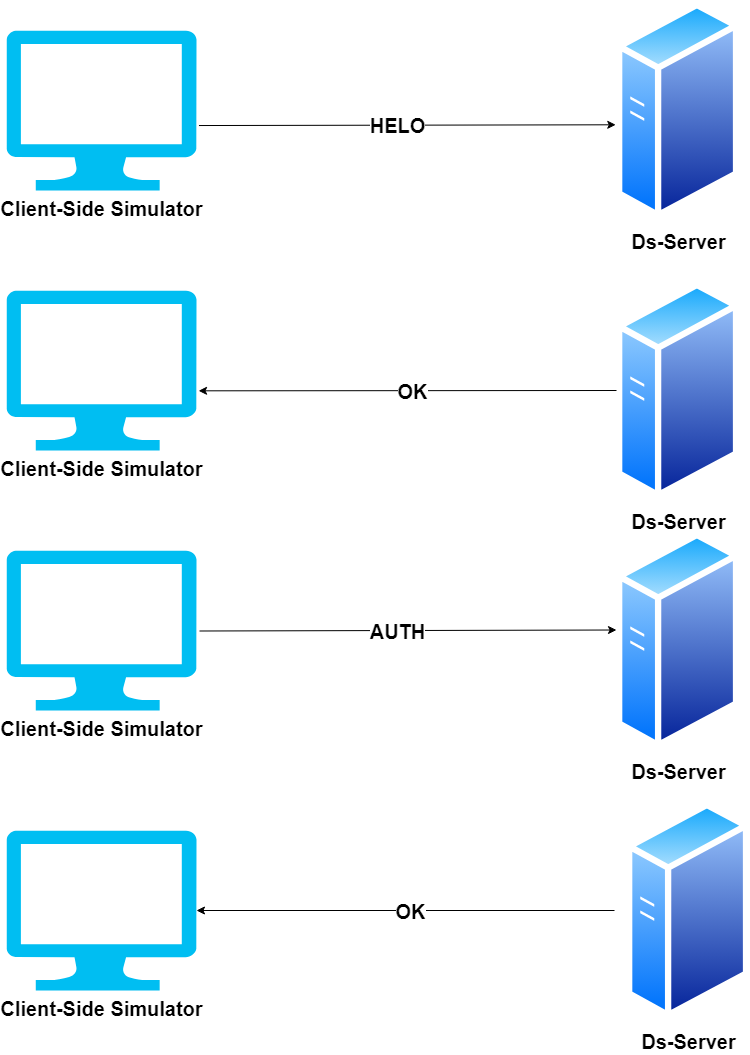
\includegraphics[width = 50mm,scale=1]{Handshake.png}
    \caption{Handshake}
    \label{Handshake}
\end{figure}




 

\subsection{Storing Server Data}
After the client-side simulator establishes a connection to the ds-server (handshake), it signals to the server that it's ready to begin scheduling jobs. The server responds by either 
\begin{itemize}
    \item Sending a job submission to the client via (JOBN)
    \item Sending information on the latest job completion via (JCPL)
\end{itemize}
upon receiving a job submission, the client-side simulator requests current server information and stores them in a hash table format with the key being the server type, e.g.(xlarge,small...etc) and the value being an array list of the server information. The workflow can be seen in figure 2
\begin{figure}[!htb]
    \centering
    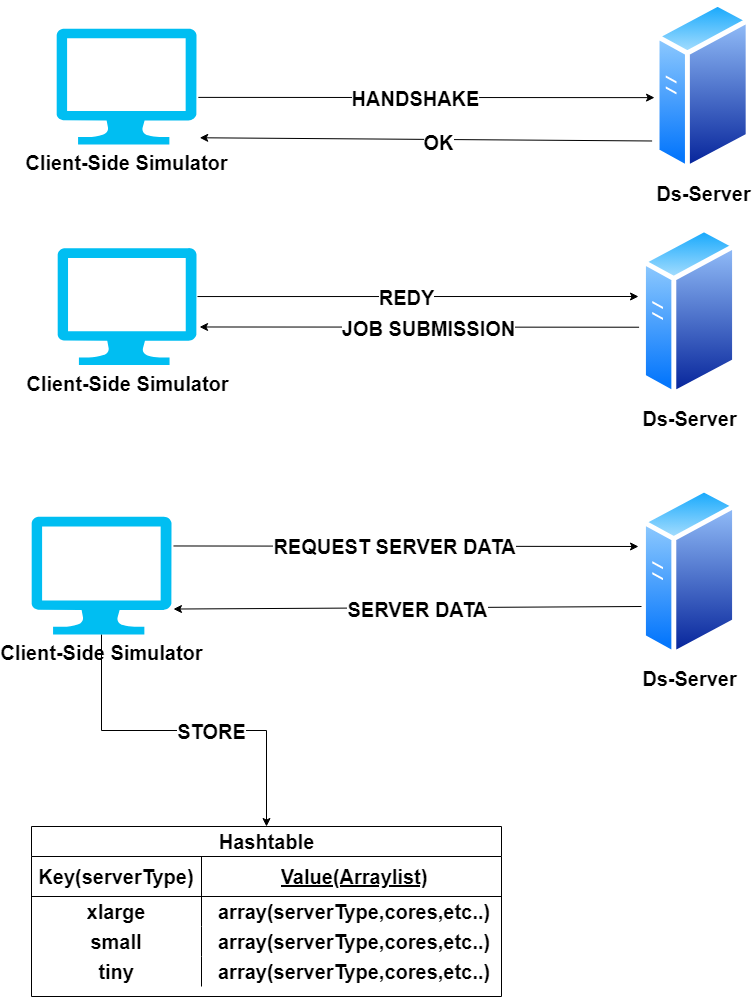
\includegraphics[width = 54mm, scale = 1]{Storing server info.png}
    \caption{Storing Server Data}
    \label{Server Data}
\end{figure}
\newpage
then the client-side simulator determines the largest server types by looking up the largest core count of each type. 
\subsection{Job Scheduler}
The client-side simulator sends a scheduling decision to the ds-server and repeats this process until all jobs have successfully been scheduled. The ds-server then sends "NONE", indicating that no more jobs are available to schedule. The client responds by sending "QUIT" to the ds-server and closing the connection.
\begin{figure}[!htb]
    \centering
    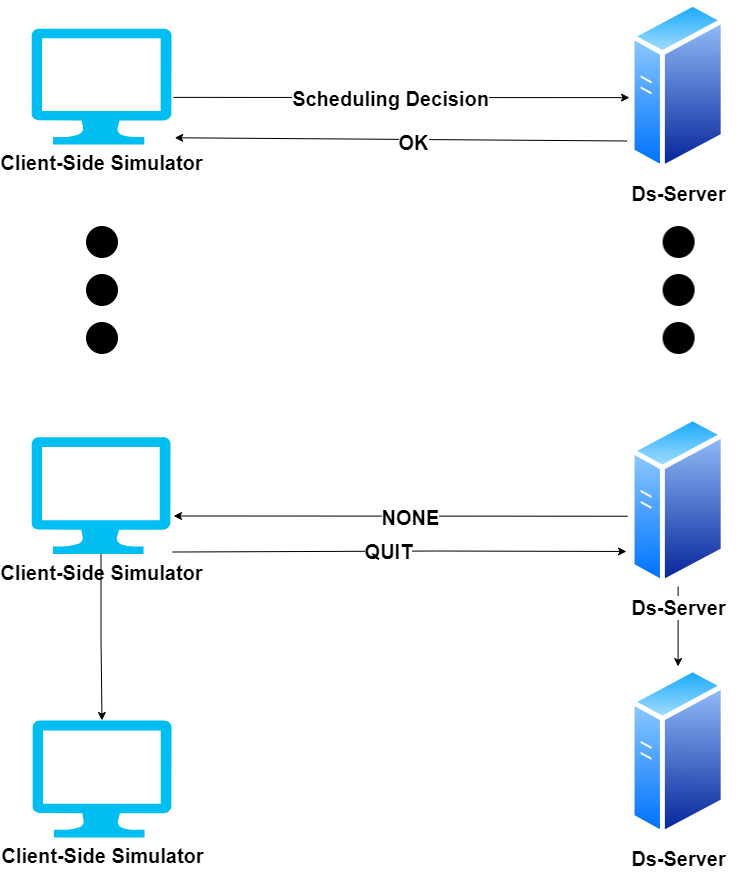
\includegraphics[width = 80mm ,scale=0.5]{Scheduling.png}
    \caption{Scheduling}
    \label{Scheduling}
\end{figure}

\label{sec:section2}

\section{Design}
\subsection{Design philosophy}
\label{sec:section3}
The design of the client-side simulator focuses on simplicity, modularity and efficiency. it implements the ds-server simulation protocols such as (GETS,SCHD) and a Largest-round robin algorithm (LRR) for scheduling jobs. The LRR algorithm was chosen for its simplicity and ease of implementation. While it may not be the most efficient in terms of resource utilisation, it provides a good starting point for implementing core functionalities to the Client-side simulator.    

\subsection{Considerations and constraints}
The design considers various constraints, such as
\begin{itemize}
    \item Network communication: The client-side simulator must establish a reliable connection with the ds-server using socket programming
    \item Responsiveness: The client-side simulator should handle all incoming messages and make informed scheduling decisions
    \item Scalability: The client-side simulator should be able to work with different server configurations
    \item Efficiency: The simulator should make optimal use of memory by implementing hash tables 
\end{itemize}

\subsection{Functionality of the Client-side simulator}
The functionality of the Client-side simulator is to act as a job scheduler for the ds-server via these steps
\begin{enumerate}
    \item Establish a connection with ds-server (Handshake)
    \item While the last message received from the server was not (NONE), signal to the ds-server that the client is ready to receive job submissions (REDY)
    \item If the message received is (JOBN), then get server information (GETS)
    \item If the message received is (JCPL), then go back to step 2
    \item Schedule a job
\end{enumerate}

\begin{figure}
    \centering
    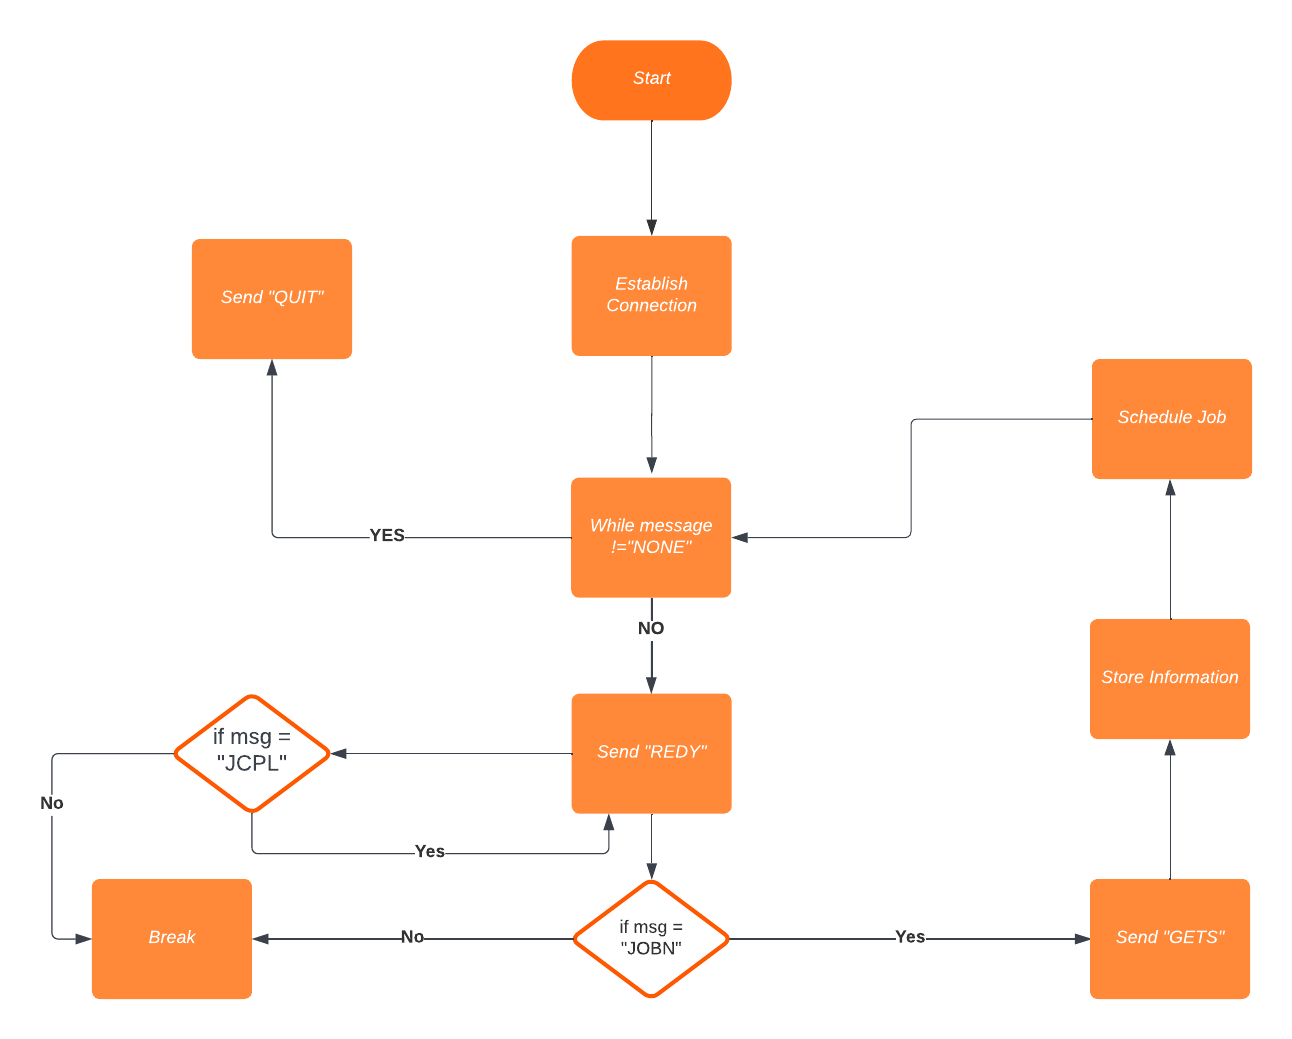
\includegraphics[width = 100mm,scale=1]{functionality flowchart - Flowchart.png}
    \caption{Functionality Flowchart}
    \label{Functionality Flowchart}
\end{figure}

\section{Implementation}
The Client-side simulator is implemented using java and uses various technologies, techniques, data structures and software libraries. The source code is divided into four classes, each responsible for a specific aspect of the simulator.
\subsection{Client Class}
The main component of the client-side simulator is the Client class\cite{Mygithubrepo}. The Client class is responsible for communications with the ds-server, other classes and the scheduling logic. This class is responsible for initialising   and managing other classes. The main method is located in this class which starts the Client-side simulator. Furthermore, this method stores server information using a hash table, as illustrated in figure 2.
\subsection{Job Class}
The job class represents the jobs submitted by the ds-server and organises them into objects that the Client class can access. Each object specifies information on the job submitted, such as Job id, cores required , memory required, disk space required. This class provides setters and getters, which are tools for accessing and modifying the content of a job submission.
\subsection{Schedule Class}
The Schedule class manages the LRR scheduling algorithm by determining the first server in the list provided by the ds-server. This class also takes input from other classes such as Job, ServerInfo to calculate the smallest index of the largest server type.
\subsection{ServerInfo Class}
While the Client class stores the given input by the ds-server, the ServerInfo class represents each server information provided by the ds-server. More importantly, the ServerInfo class takes input given from the main class (Client.class) and organises them into objects that later can be accessed.
\begin{figure}[h]
    \centering
    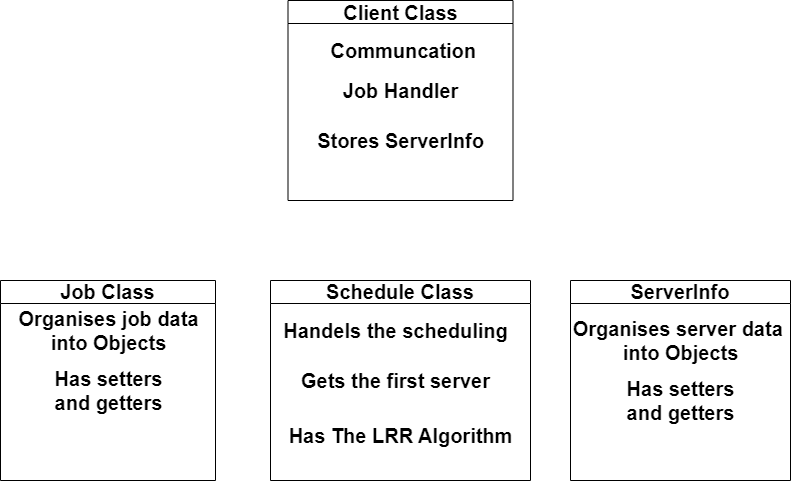
\includegraphics[width = 80mm,scale=1]{Classes.png}
    \caption{Classes}
    \label{Classes}
\end{figure}
\subsection{Technologies Used}
The Client-side simulator was built in a Linux Ubuntu using a Virtual Machine (VMware). The base operating system that used VMware is Windows 10. The text editor used to create the source code is Visual Studio Code. Various libraries were used to create the code such as
\begin{itemize}
    \item BufferedReader: Used to read input from the ds-server
    \item DataOutPutStream: Used to write commands to the ds-server such as (GETS,SCHD)
    \item IOExcepation: to handle exceptions that occurred when running the source code
    \item InputStreamReader: Used in conjunction with bufferedReader to write to the ds-server
    \item Socket: Used for socket programming and managing the connection
    \item UknownHostException: same as IOExcepation used for exception handling
    \item Arraylist: Used in conjunction with HashMap to store server information\cite{W3SArrayList}
    \item HashMap: Used to store server information in a hashtable format where the key is the ServerType and the value is an Array list that contains the server information\cite{W3SHashmap}. (see figure 2)
\end{itemize}
%----------------------------------------------------------------------------------------
%	REFERENCE LIST
%----------------------------------------------------------------------------------------
\bibliographystyle{ieeetr}
\bibliography{comp3100project}
% \printbibliography

%----------------------------------------------------------------------------------------

\end{document}
